% -*- phrases: HW2 -*-
\documentclass[pdftex,11pt]{article}
\usepackage[utf8]{inputenc}
\usepackage{tikz}	
\usepackage{graphicx}
\usepackage{listings}
\usepackage{color}
\usepackage{layout}
\usepackage{pdflscape}
\usepackage{hyperref}
\usepackage{appendix}


\hypersetup{colorlinks=true, linkcolor=blue, citecolor=blue, filecolor=blue, urlcolor=blue, pdftitle=Capstone Portfolio: Drone Flight Planning Software, pdfauthor=David Klingenberg, pdfsubject=, pdfkeywords=}

\DeclareGraphicsExtensions{.pdf,.png,.jpg}

\marginparwidth = 0pt
\marginparsep = 0pt
\topmargin = 0pt
\oddsidemargin = 0pt
\textwidth = 468pt
\textheight = 581pt
\lstset{
  language=C,                % choose the language of the code
  numbers=left,                   % where to put the line-numbers
  stepnumber=1,                   % the step between two line-numbers.        
  numbersep=5pt,                  % how far the line-numbers are from the code
  backgroundcolor=\color{white},  % choose the background color. You must add \usepackage{color}
  showspaces=false,               % show spaces adding particular underscores
  showstringspaces=false,         % underline spaces within strings
  showtabs=false,                 % show tabs within strings adding particular underscores
  tabsize=2,                      % sets default tabsize to 2 spaces
  captionpos=b,                   % sets the caption-position to bottom
  breaklines=true,                % sets automatic line breaking
  breakatwhitespace=true,         % sets if automatic breaks should only happen at whitespace
  title=\lstname,                 % show the filename of files included with \lstinputlisting;
}

 
\newcommand{\HRule}{\rule{\linewidth}{0.5mm}}

\begin{document}
\pagenumbering{gobble}
\begin{titlepage}

\begin{titlepage}
\begin{center}

% Upper part of the page. The '~' is needed because \\
% only works if a paragraph has started.

\includegraphics[width=0.15\textwidth]{./icons/04UI_Seal-Black.jpg}~\\[1cm]

\textsc{\LARGE University of Idaho}\\[1.5cm]

\textsc{\Large CS 270}\\[0.5cm]

% Title
\HRule \\[0.4cm]
{ \huge \bfseries Capstone Portfolio \\[0.4cm] }
{ \huge \bfseries Drone Mission Planning Software \\[0.4cm] }
\HRule \\[1.5cm]
\centerline{\emph{Team:}}
\centerline{Mission Control}
% Author and supervisor
\noindent
\begin{minipage}{0.4\textwidth}
\begin{flushleft} \large
\emph{Authors:}\\
David \textsc{Klingenberg}\\
Taylor \textsc{Trabun}
\end{flushleft}
\end{minipage}%
\begin{minipage}{0.4\textwidth}
\begin{flushright} \large
\vspace{20pt}
\emph{Advisors:} \\
Dr.~Bruce \textsc{Bolden}\\
Dr.~Robert \textsc{Rinker}\\
\vspace{10pt}
\emph{Customer:}\\
Brandon \textsc{Ortiz}
\end{flushright}
\end{minipage}

\vfill

% Bottom of the page
{\large \today}

\end{center}
\end{titlepage}
\end{titlepage}

\tableofcontents
\listoffigures
\listoftables

\clearpage
\pagenumbering{arabic}
\setcounter{page}{1}
\section{Team Member Contact Information}
  \begin{table}[h]
		\begin{tabular}{| l | c | p{5cm} |}
		\hline
		Name & Phone Number & Email Address\\\hline
		David Klingenberg  &  (208) 310-9657 &  bigwookiee@Gmail.com\\
		Taylor Trabun & (509) 995-0904 & trab1744@vandals.uidaho.edu\\
		\hline
	\end{tabular}
\caption{Team Member Contact Information}
\label{table:1}
\end{table}


\section{Introduction}


Software to create and upload a flight plan to a quad copter drone. The flight plan will be uploaded using xBee radio communication.\\

This project will use off-the-shelf parts.  ATMEL\textsuperscript{\textcopyright} based microcontrollers found on ardunio based open source boards is the current preference.

\subsection{Target Priorities}

\begin{table}[h]
	\begin{tabular}{c | c | p{8cm} | c}
	\hline
		 Number & Category & Need & Importance \\ \hline
		 1 & Quadcopter & Center of Gravity Refined & 5 \\
		 2 & Quadcopter & Reliable Flight & 5 \\
		 3 & Quadcopter & Functioning xBee Hardware &  4 \\
		 4 & Quadcopter & Hardware (Microcontroller) with xAPI and services to control flight & 5 \\
		 5 & Quadcopter & Controlled with XP communications &  4 \\
	   6 & Quadcopter & Autoland & 5 \\
	   7 & Software & software package for flight planning & 2\\
	   8 & Software & API for sending commands from computer & 2\\
	\end{tabular}
	\caption{Priorities}
	\label{table:2}
\end{table}

\clearpage
\section{Initial Client Interview Transcript 9/10/14}
\label{sec:clienttranscript}
%\documentclass[11pt,a4paper]{article}
%\usepackage[utf8]{inputenc}
%\usepackage{amsmath}
%\usepackage{amsfonts}
%\usepackage{amssymb}
%\title{Client Interview Transcript 9/10/14}
%\author{Team: Mission Control; Taylor Trabun and David Klingenberg}
%\begin{document}
%
%\textbf{Team: Mission Control; Taylor Trabun and David Klingenberg}
\textbf{Mentor/Client: }Brandon Ortiz

\subsection{Meetings}
We will be having weekly meetings in Brandon's office on Thursdays at 3:30 PM. These meeting will include status updates, further work on designs, troubleshooting, and assignment of tasks

\subsection{End Goal}
To have a stable and flying quadcopter that can be communicated with remotely. In addition, work done on a flight planning software (including GUI) should be underway. The project will be done in small steps, as this project requires research and development throughout.

\subsection{First Steps}
	\begin{itemize}
		\item Learn how quadcopter works
		\item Reconstruct quadcopter to be stable 
		\item Learn how to fly quadcopter
		\item Understand flight computer documentation
		\item Design communications
		\item Be sure to use xAPI
	\end{itemize}
	
\subsection{Requirements}
	\begin{itemize}
		\item Functional quadcopter (stable)
		\item Documentation of quadcopter construction
		\item Use of xAPI on arduino communication system
		\item Communication system using xBEE to communicate from computer to quadcopter
		\item Ability to send commands to quadcopter
		\item Flight planning software, including GUI
	\end{itemize}
	
\subsection{Other Notes}
Other notes from the meeting included aviation terminology, how to pair the remote control and quadcopter receiver, quick tour of controller and motor adjustments, and a quick tour of flight computer.
%\end{document}
\clearpage


\section{Meeting Agendas}
%\addcontentsline{toc}{section}{Agendas}
%\addtocounter{section}{1}

% Agenda %%%%%%%%%%%%%%%%%%%%%%%%%%%%%%%%%%%%%%%%%%%%%%%%%%%%%%%%%%%%%%%%%%%%%%%%
\subsection{Sept. 10, 2014}
{ \huge \bfseries Mission Control Team Agenda \\[0.4cm] }
{ \huge \bfseries Friday September  10, 2014.\\1500 –-  1600  in JEB   Think  Tank. \\[0.4cm] }
\vspace*{2.5mm}

{ \large \bfseries \hspace*{2 mm} Type of Meeting\\}
\hspace*{12 mm} Initial client interview.
\vspace*{1.5mm}

{ \large \bfseries \hspace*{2 mm} Attendees\\}
\hspace*{12mm} David Klingenberg\\
\hspace*{12mm} Taylor Trabun\\
\hspace*{12mm} Brandon Ortiz\\
\vspace*{1.5mm}

{ \large \bfseries \noindent Topics}
\vspace*{2.5mm}

\begin{tabular}{| l | l | l |}
  \hline
  \bfseries Topic & \bfseries Responsible & \bfseries Time (in minutes) \\ \hline
  Product  Overview  &  Brandon &  15 \\ \hline
  System  Requirements & Brandon & 15 \\ \hline
  Tasks Breakdown & Open Discussion & 15 \\ \hline
  Question \&  Answers  & Open Discussion & 25 \\ 
  \hline
\end{tabular}

\vspace*{2.5mm}
{ \large \bfseries \noindent Additional Information:}
This is our initial client interview.

\subsubsection[short]{Minutes from Friday September 10 Meeting}
Refer to \hyperref[sec:clienttranscript]{Section~\ref{sec:clienttranscript}} initial client  transcript.

% Agenda %%%%%%%%%%%%%%%%%%%%%%%%%%%%%%%%%%%%%%%%%%%%%%%%%%%%%%%%%%%%%%%%%%%%%%%%%%


% Agenda %%%%%%%%%%%%%%%%%%%%%%%%%%%%%%%%%%%%%%%%%%%%%%%%%%%%%%%%%%%%%%%%%%%%%%%%
\subsection{Sept. 18, 2014}
{ \huge \bfseries Mission Control Team Agenda \\[0.4cm] }
{ \huge \bfseries Thrusday September  18, 2014.\\1500 –-  1600  in JEB   Think  Tank. \\[0.4cm] }
\vspace*{2.5mm}

{ \large \bfseries \hspace*{2 mm} Type of Meeting\\}
\hspace*{12 mm} Initial Planning
\vspace*{1.5mm}

{ \large \bfseries \hspace*{2 mm} Attendees\\}
\hspace*{12mm} David Klingenberg\\
\hspace*{12mm} Taylor Trabun\\
\hspace*{12mm} Brandon Ortiz\\
\hspace*{12mm} Bruce Bolden\\
\vspace*{1.5mm}

{ \large \bfseries \noindent Topics}
\vspace*{2.5mm}

\begin{tabular}{| l | l | l |}
  \hline
  \bfseries Topic & \bfseries Responsible & \bfseries Time (in minutes) \\ \hline
  Progress Report  & David, Tyler &  5 \\ \hline
  System Overview & Brandon & 10 \\ \hline
  Tasks Breakdown & Open Discussion & 20 \\ \hline
  Additional Words of Wisdom & Bruce & 5 \\ \hline
  Question \&  Answers  & Open Discussion & 20 \\ 
  \hline
\end{tabular}

\vspace*{2.5mm}
{ \large \bfseries \noindent Additional Information:}


The rerouting and reconfiguring of the drone is proceeding nicely.  It progress will be shown at the meeting time. 

\subsubsection[short]{Minutes from Thursday September 18 Meeting}

\begin{itemize}
	\item 1505\indent  Meeting Started
	\item Discussed drone rebuild progress.
	\item Evaluated ESC bin for the drone.
	\begin{itemize}
		\item Refer to \hyperref[fig:partbin]{figur~\ref{fig:partbin}} in Appendix~\ref{sec:TechDraw}
	\end{itemize}  
	\item Discussed, evaluated, and illustrated the communication sequence.
	\begin{itemize}
		\item Refer to \hyperref[fig:comseq]{figur~\ref{fig:comseq}} in Appendix~\ref{sec:appUML}
	\end{itemize}
	\item 1610 \indent Meeting 
\end{itemize}
% Agenda %%%%%%%%%%%%%%%%%%%%%%%%%%%%%%%%%%%%%%%%%%%%%%%%%%%%%%%%%%%%%%%%%%%%%%%%%%


% Agenda %%%%%%%%%%%%%%%%%%%%%%%%%%%%%%%%%%%%%%%%%%%%%%%%%%%%%%%%%%%%%%%%%%%%%%%%
\subsection{Sept. 25, 2014}
{ \huge \bfseries Mission Control Team Agenda \\[0.4cm] }
{ \huge \bfseries Thrusday September 25, 2014.\\1530 –-  1630  in JEB 37\\[0.4cm] }
\vspace*{2.5mm}

{ \large \bfseries \hspace*{2 mm} Type of Meeting\\}
\hspace*{12 mm}  Status Report and  Next Week Planning
\vspace*{1.5mm}

{ \large \bfseries \hspace*{2 mm} Attendees\\}
\hspace*{12mm} David Klingenberg\\
\hspace*{12mm} Taylor Trabun\\
\hspace*{12mm} Brandon Ortiz\\
\vspace*{1.5mm}

{ \large \bfseries \noindent Topics}
\vspace*{2.5mm}

\begin{tabular}{| l | l | l |}
  \hline
  \bfseries Topic & \bfseries Responsible & \bfseries Time (in minutes) \\ \hline
  Progress Report  & David \& Tyler &  10 \\ \hline
  Demonstrations & David \& Tyler & 10 \\ \hline
  New Tasks & Open Discussion & 20 \\ \hline
  Question \&  Answers  & Open Discussion & 20 \\ 
  \hline
\end{tabular}

\vspace*{2.5mm}
{ \large \bfseries \noindent Additional Information:}

\subsubsection[short]{Minutes from Thursday September 25 Meeting}
\begin{itemize}
	\item 1530 \indent Meeting Start
	\item Discussed LCD use on Arduinos.
	\item Reviewed TUN  packets.
	\item  Status updates
	\begin{itemize}
		\item Things moving along.
		\item Getting closer to flying possibly  next Thursday.
	\end{itemize}
	\item xBee discussion on how to connect.
	\item Evaluated future problems.
	\begin{itemize}
		\item  Gyros and accelerometers need to be implemented separately from the flight computer.
	\end{itemize}
	\item 1630 \indent Meeting Ended
\end{itemize}	

\clearpage
% Agenda %%%%%%%%%%%%%%%%%%%%%%%%%%%%%%%%%%%%%%%%%%%%%%%%%%%%%%%%%%%%%%%%%%%%%%%%%%

% Agenda %%%%%%%%%%%%%%%%%%%%%%%%%%%%%%%%%%%%%%%%%%%%%%%%%%%%%%%%%%%%%%%%%%%%%%%%
\subsection{Oct. 2, 2014}
{ \huge \bfseries Mission Control Team Agenda \\[0.4cm] }
{ \huge \bfseries Thrusday October 2, 2014.\\1530 –-  1630  in JEB 37\\[0.4cm] }
\vspace*{2.5mm}

{ \large \bfseries \hspace*{2 mm} Type of Meeting\\}
\hspace*{12 mm}  Status Report and  Next Week Planning
\vspace*{1.5mm}

{ \large \bfseries \hspace*{2 mm} Attendees\\}
\hspace*{12mm} David Klingenberg\\
\hspace*{12mm} Taylor Trabun\\
\hspace*{12mm} Brandon Ortiz\\
\vspace*{1.5mm}

{ \large \bfseries \noindent Topics}
\vspace*{2.5mm}

\begin{tabular}{| l | l | l |}
  \hline
  \bfseries Topic & \bfseries Responsible & \bfseries Time (in minutes) \\ \hline
  Progress Report  & David \& Tyler &  10 \\ \hline
  Demonstrations & David \& Tyler & 10 \\ \hline
  New Tasks & Open Discussion & 20 \\ \hline
  Question \&  Answers  & Open Discussion & 20 \\ 
  \hline
\end{tabular}

\vspace*{2.5mm}
{ \large \bfseries \noindent Additional Information:}

\subsubsection[short]{Minutes from Thursday October 2 Meeting}
\begin{itemize}
	\item 1530 \indent Meeting Start
	\item  Status updates.
	\begin{itemize}
		\item Taylor has one-way communications working.
		\item  David finished a prototype for the ECS bin.
		\begin{itemize}
			\item Bin needs its weight reduced.
			\item ECS cables need to be lengthened.
		\end{itemize}
	\end{itemize}
	\item  To 
	\begin{itemize}
		\item Taylor will attempt to get XP comm working.
		\item David will finish quadcopter.
		\item Get a new adrenal for running a second xBee  radio.
		\item Solder new LCD board.
	\end{itemize}
	\item xBee  Configuration notes.
	\begin{itemize}
		\item Use XCTU tool for configuration.
		\item Need FID drivers installed for XCTU tool.
	\end{itemize}
	\item 1630 \indent Meeting Ended
\end{itemize}	

% Agenda %%%%%%%%%%%%%%%%%%%%%%%%%%%%%%%%%%%%%%%%%%%%%%%%%%%%%%%%%%%%%%%%%%%%%%%%%%

% Agenda %%%%%%%%%%%%%%%%%%%%%%%%%%%%%%%%%%%%%%%%%%%%%%%%%%%%%%%%%%%%%%%%%%%%%%%%
\subsection{Oct. 9, 2014}
{ \huge \bfseries Mission Control Team Agenda \\[0.4cm] }
{ \huge \bfseries Thrusday October 9, 2014.\\1530 –-  1630  in JEB 37\\[0.4cm] }
\vspace*{2.5mm}

{ \large \bfseries \hspace*{2 mm} Type of Meeting\\}
\hspace*{12 mm}  Status Report and  Next Week Planning
\vspace*{1.5mm}

{ \large \bfseries \hspace*{2 mm} Attendees\\}
\hspace*{12mm} David Klingenberg\\
\hspace*{12mm} Taylor Trabun\\
\hspace*{12mm} Brandon Ortiz\\
\vspace*{1.5mm}

{ \large \bfseries \noindent Topics}
\vspace*{2.5mm}

\begin{tabular}{| l | l | l |}
  \hline
  \bfseries Topic & \bfseries Responsible & \bfseries Time (in minutes) \\ \hline
  Progress Report  & David \& Tyler &  10 \\ \hline
  Demonstrations & David \& Tyler & 10 \\ \hline
  New Tasks & Open Discussion & 20 \\ \hline
  Question \&  Answers  & Open Discussion & 20 \\ 
  \hline
\end{tabular}

\vspace*{2.5mm}
{ \large \bfseries \noindent Additional Information:}

\subsubsection[short]{Minutes from Thursday October 9 Meeting}
\begin{itemize}
	\item 1530 \indent Meeting Start
	\item Update
	\begin{itemize}
		\item  Taylor is preparing for snapshot day.
		\item David
		\begin{itemize}
			\item Quadcopter rebuilt.
			\item Simple xBee terminals working between two computers.
		\end{itemize}
	\end{itemize}
	\item New Resources
		\begin{itemize}
			\item UAV control paper with GUI design example.
			\item Survey of UAV papers.
		\end{itemize}
	\item Action Items
	\begin{itemize}
		\item David will experiment with PWM and the quadcopter and  portfolio.
		\item Taylor will work on poster for snapshot day and continue working on communications.
	\end{itemize}
	\item Test Flight
	\begin{itemize}
		\item  Quadcopter has severe drift forward. David will work on solution.
	\end{itemize}
	\item 1630 \indent Meeting Ended
\end{itemize}	


\clearpage
% Agenda %%%%%%%%%%%%%%%%%%%%%%%%%%%%%%%%%%%%%%%%%%%%%%%%%%%%%%%%%%%%%%%%%%%%%%%%%%

\clearpage
\appendix
\appendixpage	
\addappheadtotoc

\section{Miscellaneous UML Charts}
\label{sec:appUML}
\begin{figure}[!h]
	\centering
		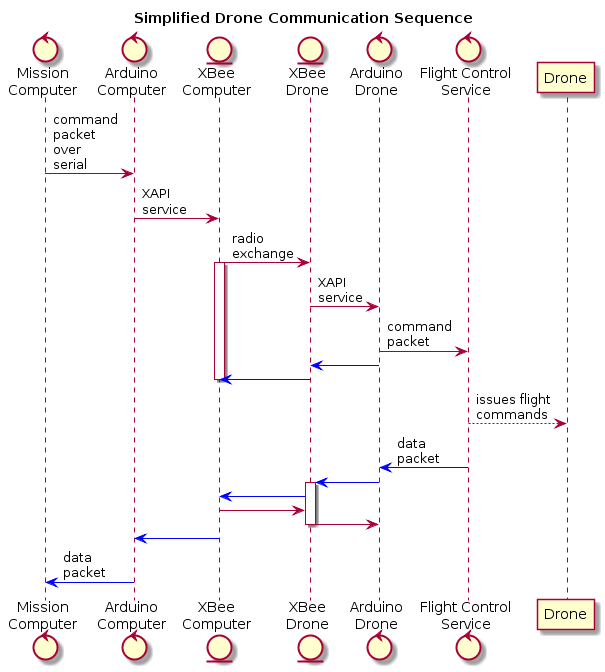
\includegraphics[width=0.5\textwidth]{./plantUML/droneControlSequence.png}
	\caption{Communication Sequence}
	\label{fig:comseq}
\end{figure}

\clearpage
\section{ATMEL\textsuperscript{\textcopyright} Microcontrollers}
\label{sec:appATMEL}
\begin{figure}[!h]
	\centering
		\includegraphics[width=.8\textwidth]{./additionalPDF/Atmel-644.pdf}
	\caption{ATmega644}
	\label{fig:ATmega644}
\end{figure}

\begin{figure}[!h]
	\centering
		\includegraphics[width=.8\textwidth]{./additionalPDF/Atmel-2560.pdf}
	\caption{ATmega2560}
	\label{fig:ATmega2560}
\end{figure}

\clearpage

\section{Technical Drawings}
\label{sec:TechDraw}

\begin{figure}[!h]
	\centering
		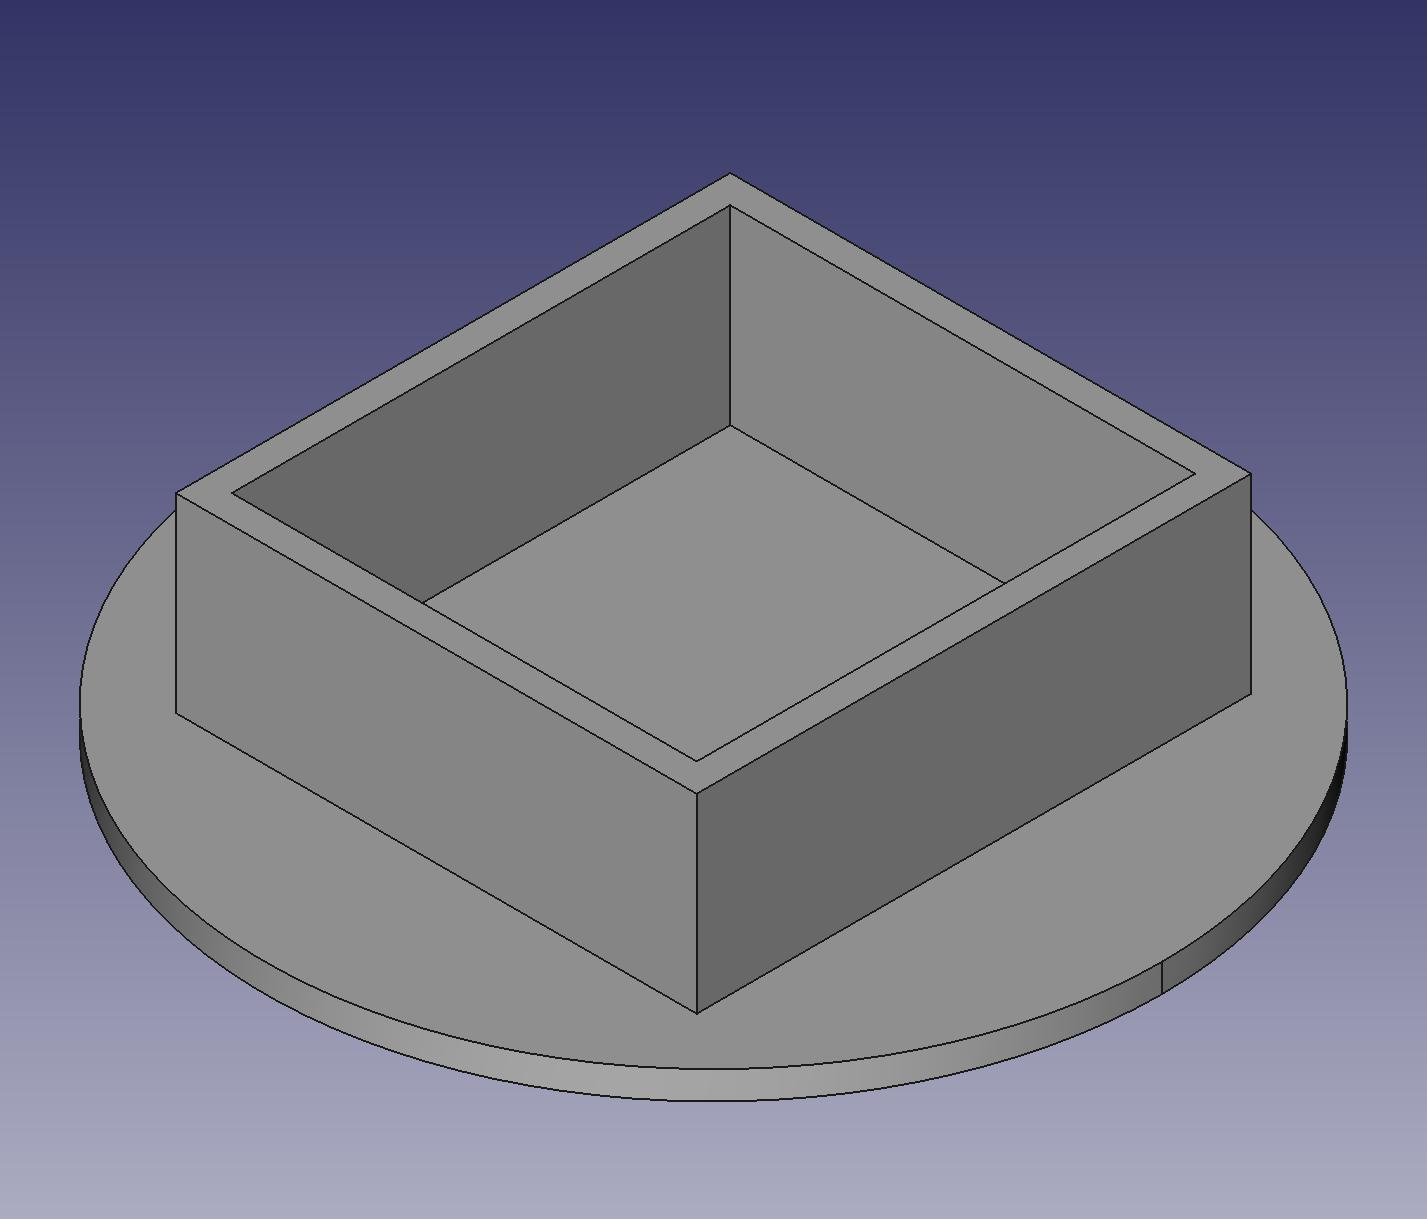
\includegraphics[width=.5\textwidth]{./graphics/partbin.jpg}
	\caption{Electronic speed controller part bin}
	\label{fig:partbin}
\end{figure}

\end{document}
%%%%%%%%%%%%%%%%%%%%%%%%%%%%%%%%%%%%%%%% END %%%%%%%%%%%%%%%%%%%%%%%%%%%%%%%%%%%%%%%%%%%%%%%%%%